%-----------------------------------------------------------------
%	RESULTS
%	!TEX root = ./../main.tex
%-----------------------------------------------------------------
\section{Implementation with a Genetic Algorithm}\label{sec:implementation}\nocite{Sean2010}
\subsection{Methodology of a Genetic Algorithm}\label{sec:genetic-alg-structure}
The Genetic Algorithm was invented by John Holland at the University of Michigan in the 1970s. This evolutionary algorithm consists on iterating through fitness assessment, recombination, and population reassembly.

In the recombination process, we select two parents from the original population, cross them over with one another, and mutate the results. The children are then reassembled into the original population (the way to do this varies from author to author).

\bigskip
\textcite{Zapfel2010} go into great detail on how each of the components of the algorithm affect the solution of the problem. In figure \ref{fig:structure} we can see a simple diagram on how the Genetic Algorithm is structured and how each of the operations depends on the specific problem one wants to tackle.
\begin{figure}[H]
	\centering
	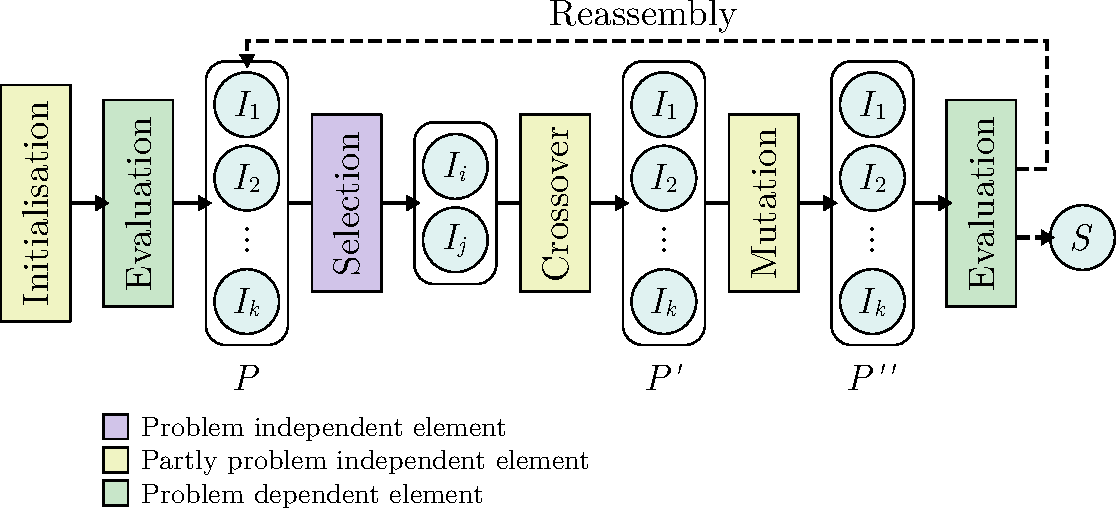
\includegraphics[width=0.8\textwidth]{images/genetic-algorithm}
	\caption{Structure of a Genetic Algorithm}
	\label{fig:structure}
\end{figure}

One might wonder why initialisation, crossover, and mutation are marked partly problem dependent here. The reason is that in Genetic Algorithms, different encodings can be used to represent individuals. By using simple or generic encodings, like binary or permutation, one can use standard genetic operators for crossover and mutation. Hence those operators are referred to as partly problem dependent. The main advantage is the applicability of generic crossover and mutation operators, i.e. no problem specific operators must be developed.

%-----------------------------------------------------------------
\subsection{Computational structure of the program}\label{sec:program}
First of all, we need to decide the programming language we will use to implement the Genetic Algorithm. I decided to use Python 3, as I am more experienced with it, and because it would allow me to tweak the program and play with the different parameters without focusing too much on the technical side of things.

One of the main advantages of using an object-oriented programming language like Python is the ability to use classes to group each individual with its properties (sequence and fitness) in an organised and straightforward way. In \cref{sn:class} we can see the \inline{BoardPermutation} class we will use to store each one of the individuals or \inline{board}s.

\begin{lstlisting}[label=sn:class, caption=Definition of the \inline{BoardPermutation} class]
class BoardPermutation:
	def __init__(self):
		self.sequence = None
		self.fitness = None
	def set_sequence(self, val):
		self.sequence = val
	def set_fitness(self, fitness):
		self.fitness = fitness
	def get_attr(self):
		return { 'sequence' : sequence, 'fitness' : fitness }
\end{lstlisting}

In the following sections we will see how \inline{sequence} and \inline{fitness} are defined.

%-----------------------------------------------------------------
\subsection{Initialisation of the population}\label{sec:init}

Now that we know the computational structure of the individuals, we can work out a function to generate each of the individuals that constitute the initial population. In \cref{sn:generate_chromosome} we can see how we define our \inline{generate_chromosome()} function. What the function does is generate an ordered array from \inline{0} to \inline{N_QUEENS} (as in \inline{[0 1 2 3 ... N_QUEENS]}), and then shuffle the elements to create different permutations. For the sake of academic rigour, as is usual with Genetic Algorithms, we call each individual a chromosome.

\begin{lstlisting}[label=sn:generate_chromosome, caption=Function to generate a single individual]
def generate_chromosome():
	# Randomly generates a sequence of board states.
	init_distribution = np.arange(N_QUEENS)
	np.random.shuffle(init_distribution)
	return init_distribution
\end{lstlisting}

Notice that we are using Python's \inline{numpy} library, which makes our program run as fast\footnote{Provided we know how to make an efficient program (which is probably not the case).} as if it used native C. This is, as is usual with powerful and fast libraries, because \inline{numpy} is written in C.

All we have to do now is to generate the initial population. The implementation is straightforward: we create a list of \inline{population_size} objects of class \inline{BoardPermutation}. Then all we need to do is to set the sequence and the fitness of each board using the \inline{generate_chromosome()} and \inline{assess_fitness()} functions, respectively. This is clearly illustrated in \cref{sn:generate_population}.

\begin{lstlisting}[label=sn:generate_population, caption=Population initialization function]
def generate_population(population_size = 100):
	# Create the different boards
	population = [BoardPermutation() for i in range(population_size)]
	for i in range(population_size):
		population[i].set_sequence(generate_chromosome())
		population[i].set_fitness(assess_fitness(population[i].sequence))
	return population
\end{lstlisting}

%-----------------------------------------------------------------
\subsection{Evaluation: fitness function}\label{sec:fitness}

The evaluation function determines the quality of a candidate solution. In metaheuristics this is usually called fitness function. The fitness value of a proposed solution is needed for the selection process and eventually finding the final solution of our problem.

As we mentioned before, the assessment of the fitness of a solution is a problem dependent element. In \cref{sec:representation} and \cref{sec:init} we discussed how we only worked with permutations of an array of non-repeated consecutive numbers. This eases the calculation of the fitness quite a bit.

Since the queens are by definition in different rows and columns, we only have to check if a queen attacks another one diagonally. We could do this by iterating on the diagonal cells of any given queen and check if there's a queen in any of the cells, but this is a bit complex to program. We found that the easiest way to check if two queens attack each other is to check if
\begin{align}
	\abs{ x_{i} - x_{j} } \equiv \abs{ y_{i} - y_{j} }
\end{align}
that is, when the two queens' vertices define a square, as depicted in figure \ref{fig:4queens-attack}.

\begin{figure}[H]
	\centering
	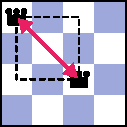
\includegraphics[height=0.18\textwidth]{images/4queens-attack}
	\caption{Example of a queen attacking another queen}
	\label{fig:4queens-attack}
\end{figure}

In \cref{sn:assess_fitness} we can see our implementation of the fitness function. In it we count the amount of clashed produced in any given board, then we return \inline{MAX_FIT - clashes}. In this problem, \inline{MAX_FIT} is $N (N-1)$; the reason behind this is really simple. We can think of the queens as a set of $N$ vertices; in a $K_{N}$ graph, the amount of edges is $v (v-1)/ 2$, where edges connect queens that don't clash with one another. The reason behind the $\times 2$ factor is that we count clashes twice in our loop; this doesn't matter as long as our fitness function is well defined and behaves in a controlled way.

\begin{lstlisting}[label=sn:assess_fitness, caption=Fitness function]
def assess_fitness(chromosome = None):
	clashes = 0
	# Calculate diagonal clashes
	for i in range(len(chromosome)):
		for j in range(len(chromosome)):
			if ( i != j):
				dx = abs(i-j)
				dy = abs(chromosome[i] - chromosome[j])
				if(dx == dy):
					clashes += 1
	return (MAX_FIT - clashes)
\end{lstlisting}

%-----------------------------------------------------------------
\subsection{Recombination process}\label{sec:recombination}
This is probably the most important part of the whole Genetic Algorithm. This is the part where we need to choose if we want to focus on exploitation (corresponding to intensification) or exploration (corresponding to diversification). This is not an easy task, because in an ideal scenario, we want the balance between both; as \textcite{Stutzle1999} puts it
\begin{quotation}
	\emph{A metaheuristic will be successful on a given optimization problem if it can provide a balance between the exploitation of the accumulated search experience and the exploration of the search space to identify regions with high quality solution in a problem specific, near optimal way.}
\end{quotation}

Not only that, but using a population of permutation individuals as a trade-off of having an easier fitness function, the crossover function has to be modified to avoid getting an invalid children when recombining two parents (e.g., \inline{[1 1 0 3]}). Although most texts deal with crossovers in the most generalised manner, some do make this distinction and tweak the classical algorithms to impede such children; such as \textcite{Gendreau2010}, and \textcite{Goldberg1989}. The same is true for the mutation function, although the workaround is fairly straightforward.

%-----------------------------------------------------------------
\subsubsection*{Parent selection}%\nocite{Gendreau2010}
As mentioned before, the parent selection is trivial, as it does not depend on the structure our individuals; the only important parameter is their fitness.

The usual selection methods involve ranking in some fashion all individuals by their fitness. The most widely used method is the Fitness-Proportionate Selection, also known as Roulette Selection. This method is discussed in detail by \textcite{Sean2010} and \textcite{Gendreau2010}; in short it selects individuals with higher fitness more often (this involves defining a selection pressure, or a survival function).

The method we will use, however, is the Tournament Selection. In this selection method a set of $\tau$ (this is called the Tournament Size) chromosomes are chosen and compared, the best one being selected for parenthood. Our implementation can be seen in \cref{sn:tournament}.

\begin{lstlisting}[label=sn:tournament, caption=Parent selection using a Tournament Selection]
def get_parent(population = None):
	# Get parent using a Tournament Selection algorithm
	best_board = random.randint(0, len(population) - 1)
	tournament_size = 2
	for i in range(1,tournament_size):
		next_board = random.randint(0, len(population) - 1)
		if ( population[next_board].fitness > population[best_board].fitness ):
			best_board = next_board
	return best_board
\end{lstlisting}

Using a Tournament Selection over a Fitness-Proportionate Selection has quite a number of advantages. First of all, it can deal with situations where there is no formal objective fitness function (needed to define the selection pressure), as it is not sensitive to how it is defined; it only needs the fitness value itself. Second, it is not a complex method, leading to very fast computation times. Last but not least, it can be finely tuned to our liking; allowing us to be more exploratory or exploitatory.

In the Genetic Algorithm, the most popular setting is $\tau = 2$; this approach has similar properties to Fitness-Proportionate Selection. This value for the Tournament Size leads to a fairly exploratory algorithm, but using bigger values makes the algorithm too exploitatory, which can lead to very slow (or very fast, depending on the initial population\footnote{This can be understood in terms of Lyapunov's instability principle.}) convergence.

Anyhow, we are interested in finding the balance between exploration and exploitation, so we'll stick with $\tau = 2$, and try to tune our algorithm playing with other parameters of the algorithm, which we will discuss with more detail in \cref{sec:parameter-control}).

%-----------------------------------------------------------------
\subsubsection*{Ordered crossover}\nocite{Goldberg1989}

Under a standard Two-Point Crossover, two parents are aligned and two crossing points are picked uniformly at random. These two points define a matching region, which are swapped between the two parents, giving place to two children:

\begin{align}
	\mqty{
	P_{1}: & \inline{[ 0 4 | 2 3 1 | 5 ]} \\
	P_{2}: & \inline{[ 5 0 | 2 1 4 | 3 ]}
	}
	\, \mapsto \,
	\mqty{
	P_{1}': & \inline{[ 0 4 | 2 1 4 | 5 ]} \\
	P_{2}': & \inline{[ 5 0 | 2 3 1 | 3 ]}
	 }
\end{align}

The first thing we notice is that this simple crossover has led to two invalid individuals under our permutation representation, just as we warned in \cref{sec:recombination}. This will surely be the case for most crossovers. So let's find a better suited crossover function for the problem in our hands.

The Partially-Matched Crossover, or PMX, tries to solve this problem. Its philosophy is very similar to that of the Two-Point Crossover: two points are randomly selected to define a matching region. The difference is that the matching region defines a position-by-position interchange mapping. Let's see this with an example:

\begin{align}
	\mqty{
	P_{1}: & \inline{[ 0 4 | 2 3 1 | 5 ]} \\
	P_{2}: & \inline{[ 5 0 | 2 1 4 | 3 ]}
	}
	\, \mapsto \,
	\mqty{
	P_{1}': & \inline{[ 0 4 | 2 1 3 | 5 ]} \\
	P_{2}': & \inline{[ 5 0 | 2 3 1 | 4 ]}
	 }
\end{align}


\todo[inline]{Reimplement PMX.}

\begin{lstlisting}[label=sn:, caption={Ordered crossover function, as described by \textcite{Goldberg1989}}]
def ordered_crossover(ind1 = None, ind2 = None):
def ordered_crossover(ind1 = None, ind2 = None):
	# Ordered crossover
	a, b = random.sample(range(N_QUEENS), 2)
	if a > b:
			a, b = b, a
	holes1, holes2 = [True]*N_QUEENS, [True]*N_QUEENS
	for i in range(N_QUEENS):
		if i < a or i > b:
			holes1[ind2[i]] = False
			holes2[ind1[i]] = False
	# We must keep the original values somewhere before scrambling everything
	temp1, temp2 = ind1, ind2
	k1 , k2 = b + 1, b + 1
	for i in range(N_QUEENS):
		if not holes1[temp1[(i + b + 1) % N_QUEENS]]:
			ind1[k1 % N_QUEENS] = temp1[(i + b + 1) % N_QUEENS]
			k1 += 1
		if not holes2[temp2[(i + b + 1) % N_QUEENS]]:
			ind2[k2 % N_QUEENS] = temp2[(i + b + 1) % N_QUEENS]
			k2 += 1
	# Swap the content between a and b (included)
	for i in range(a, b + 1):
		ind1[i], ind2[i] = ind2[i], ind1[i]
\end{lstlisting}

%-----------------------------------------------------------------
\subsubsection*{Mutation}\nocite{Zapfel2010}

\todo[inline]{Explain mutation.}

\begin{lstlisting}[label=sn:mutate, caption=Mutation function]
def mutate(board = None):
	# Mutate a board using a mask
	if random.random() < MUTATE :
		a, b = random.randint(0, N_QUEENS - 1), random.randint(0, N_QUEENS - 1)
		while (b == a): # To ensure a true mutation
			b = random.randint(0, N_QUEENS - 1)
		population[board].sequence[a], population[board].sequence[b] = population[board].sequence[b], population[board].sequence[a]
\end{lstlisting}

%-----------------------------------------------------------------
\subsubsection*{Reassembly of the population}\nocite{Zapfel2010}

\todo[inline]{Rewrite this section. We could move to the top?}

There are several replacement schemes, where the most popular are:
\begin{itemize}
	\item generational replacement.
	\item steady-state replacement.
\end{itemize}

In generational replacement the new generation supersedes the old generation. But this replacement scheme has a big disadvantage. If one replaces the whole generation the risk of dismissing a very promising solution is high. So, De Jong invented a concept called elitism where the most promising solution is always kept in the population (cf. [168]). The next step is to keep not only one but n elite solutions, this is called n-elitism. The other extreme is not to keep only one solution but to replace only one solution. This replacement scheme is called steady-state replacement (cf. [168]). In [176] steady-state replacement is defined differently. There, not only one solution is replaced but multiple solutions, they generalize the idea. But whether only a single solution or multiple solutions are replaced, by using steady state replacement one must define which solutions are replaced (worst, random, double, parents...)

Our implementation uses steady-state replacement of the parents.

%-----------------------------------------------------------------
\subsection{Evaluation: stop condition}\label{sec:stop-cond}

\todo[inline]{Expand this section.}

\begin{lstlisting}[label=sn:find_good_queen, caption=Function to stop the program when we find a good solution]
def find_good_queen(population = None):
	# Look for a good board
	for board in range(len(population)):
		if ( population[board].fitness == MAX_FIT ):
			print("Found a non-fundamental solution.")
			print( "Q",  board, ":", population[board].sequence, "fitness:", population[board].fitness )
			return True
\end{lstlisting}

Since we are using a steady-state replacement of the parents, most of our functions just do operations within the population itself; the \emph{crucial} return value in the algorithm is the return of the \inline{find_good_queen()} function. As we'll see later, the Genetic Algorithm stops when \inline{find_good_queen()} returns the boolean \inline{True}.

%-----------------------------------------------------------------
\subsection{The Genetic Algorithm}\label{sec:genetic-algorithm}
Now we have all the ingredients to define our main \inline{genetic_algorithm()} function. This function just calls all the other functions in the usual order (remember figure \ref{fig:structure}), so it's quite self-explanatory and easy to understand. We can see our implementation in \cref{sn:genetic_algorithm}.

\begin{lstlisting}[label=sn:genetic_algorithm, caption=The Genetic Algorithm]
def genetic_algorithm(MAX_ITER):
	for iteration in range(MAX_ITER):
		print(" #"*5 ,"Genetic generation :", iteration, "#"*5)
		# Select parents
		parent1 = get_parent(population)
		parent2 = get_parent(population)
		ordered_crossover(population[parent1].sequence, population[parent2].sequence)
		# Mutate children
		if(MUTATE_FLAG):
			mutate(parent1)
			mutate(parent2)
		# Reassess fitness
		population[parent1].set_fitness(assess_fitness(
			population[parent1].sequence))
		population[parent2].set_fitness(assess_fitness(
			population[parent2].sequence))
		if find_good_queen(population):
			break
\end{lstlisting}

To run the Genetic Algorithm we just need to do three simple things: (i) start our initial population, (ii) tell the program it hasn't found a solution yet, (ii) execute the algorithm until it finds a good solution or \inline{MAX_ITER} is reached:

\begin{lstlisting}[label=sn:main, caption=Instructions needed to perform the Genetic Algorithm]
population = generate_population(POPULATION)
good = False
genetic_algorithm(MAX_ITER)
\end{lstlisting}

Below we can see a typical output of running our Python program. In particular, we have run \inline{python n-queens.py 8 200} to solve the 8 Queens Problem with an initial population of 200 individuals:
\renewcommand{\lstlistingname}{Snippet}
\begin{lstlisting}[style=output, label=out:n-queens8-200]
# # # # # Genetic generation : 0 #####
# # # # # Genetic generation : 1 #####
# # # # # Genetic generation : 2 #####
# # # # # Genetic generation : 3 #####
Found a non-fundamental solution.
Q 126 : [1 6 4 7 0 3 5 2] fitness: 56
\end{lstlisting}

We found a valid solution (depicted in figure \ref{fig:8queens-example}) in fourth generation of the algorithm.
\begin{figure}[H]
	\centering
	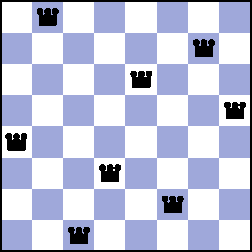
\includegraphics[height=0.36\textwidth]{images/8queens-example}
	\caption{A single solution for the 8 Queens Problem}
	\label{fig:8queens-example}
\end{figure}
